%%=============================================================================
%% Voorbereiding op het onderzoek
%%=============================================================================

\chapter{Data Vault: data warehousing}
\label{ch:dvmodel}
In dit hoofdstuk wordt een data warehouse opgebouwd aan de hand van data vault. Elke laag van de architectuur (en de bijhorende ETL) wordt aan bod gebracht. Op het einde van dit hoofdstuk moet er via een rapporteringsomgeving kunnen verbonden worden met een ontworpen data mart, gebaseerd op een data warehouse ontworpen met de data vault methodologie, om de benodigde gegevens te kunnen opvragen.

\newpage
\section{Overzicht datamodel}
\begin{figure}[h]
	\centering
	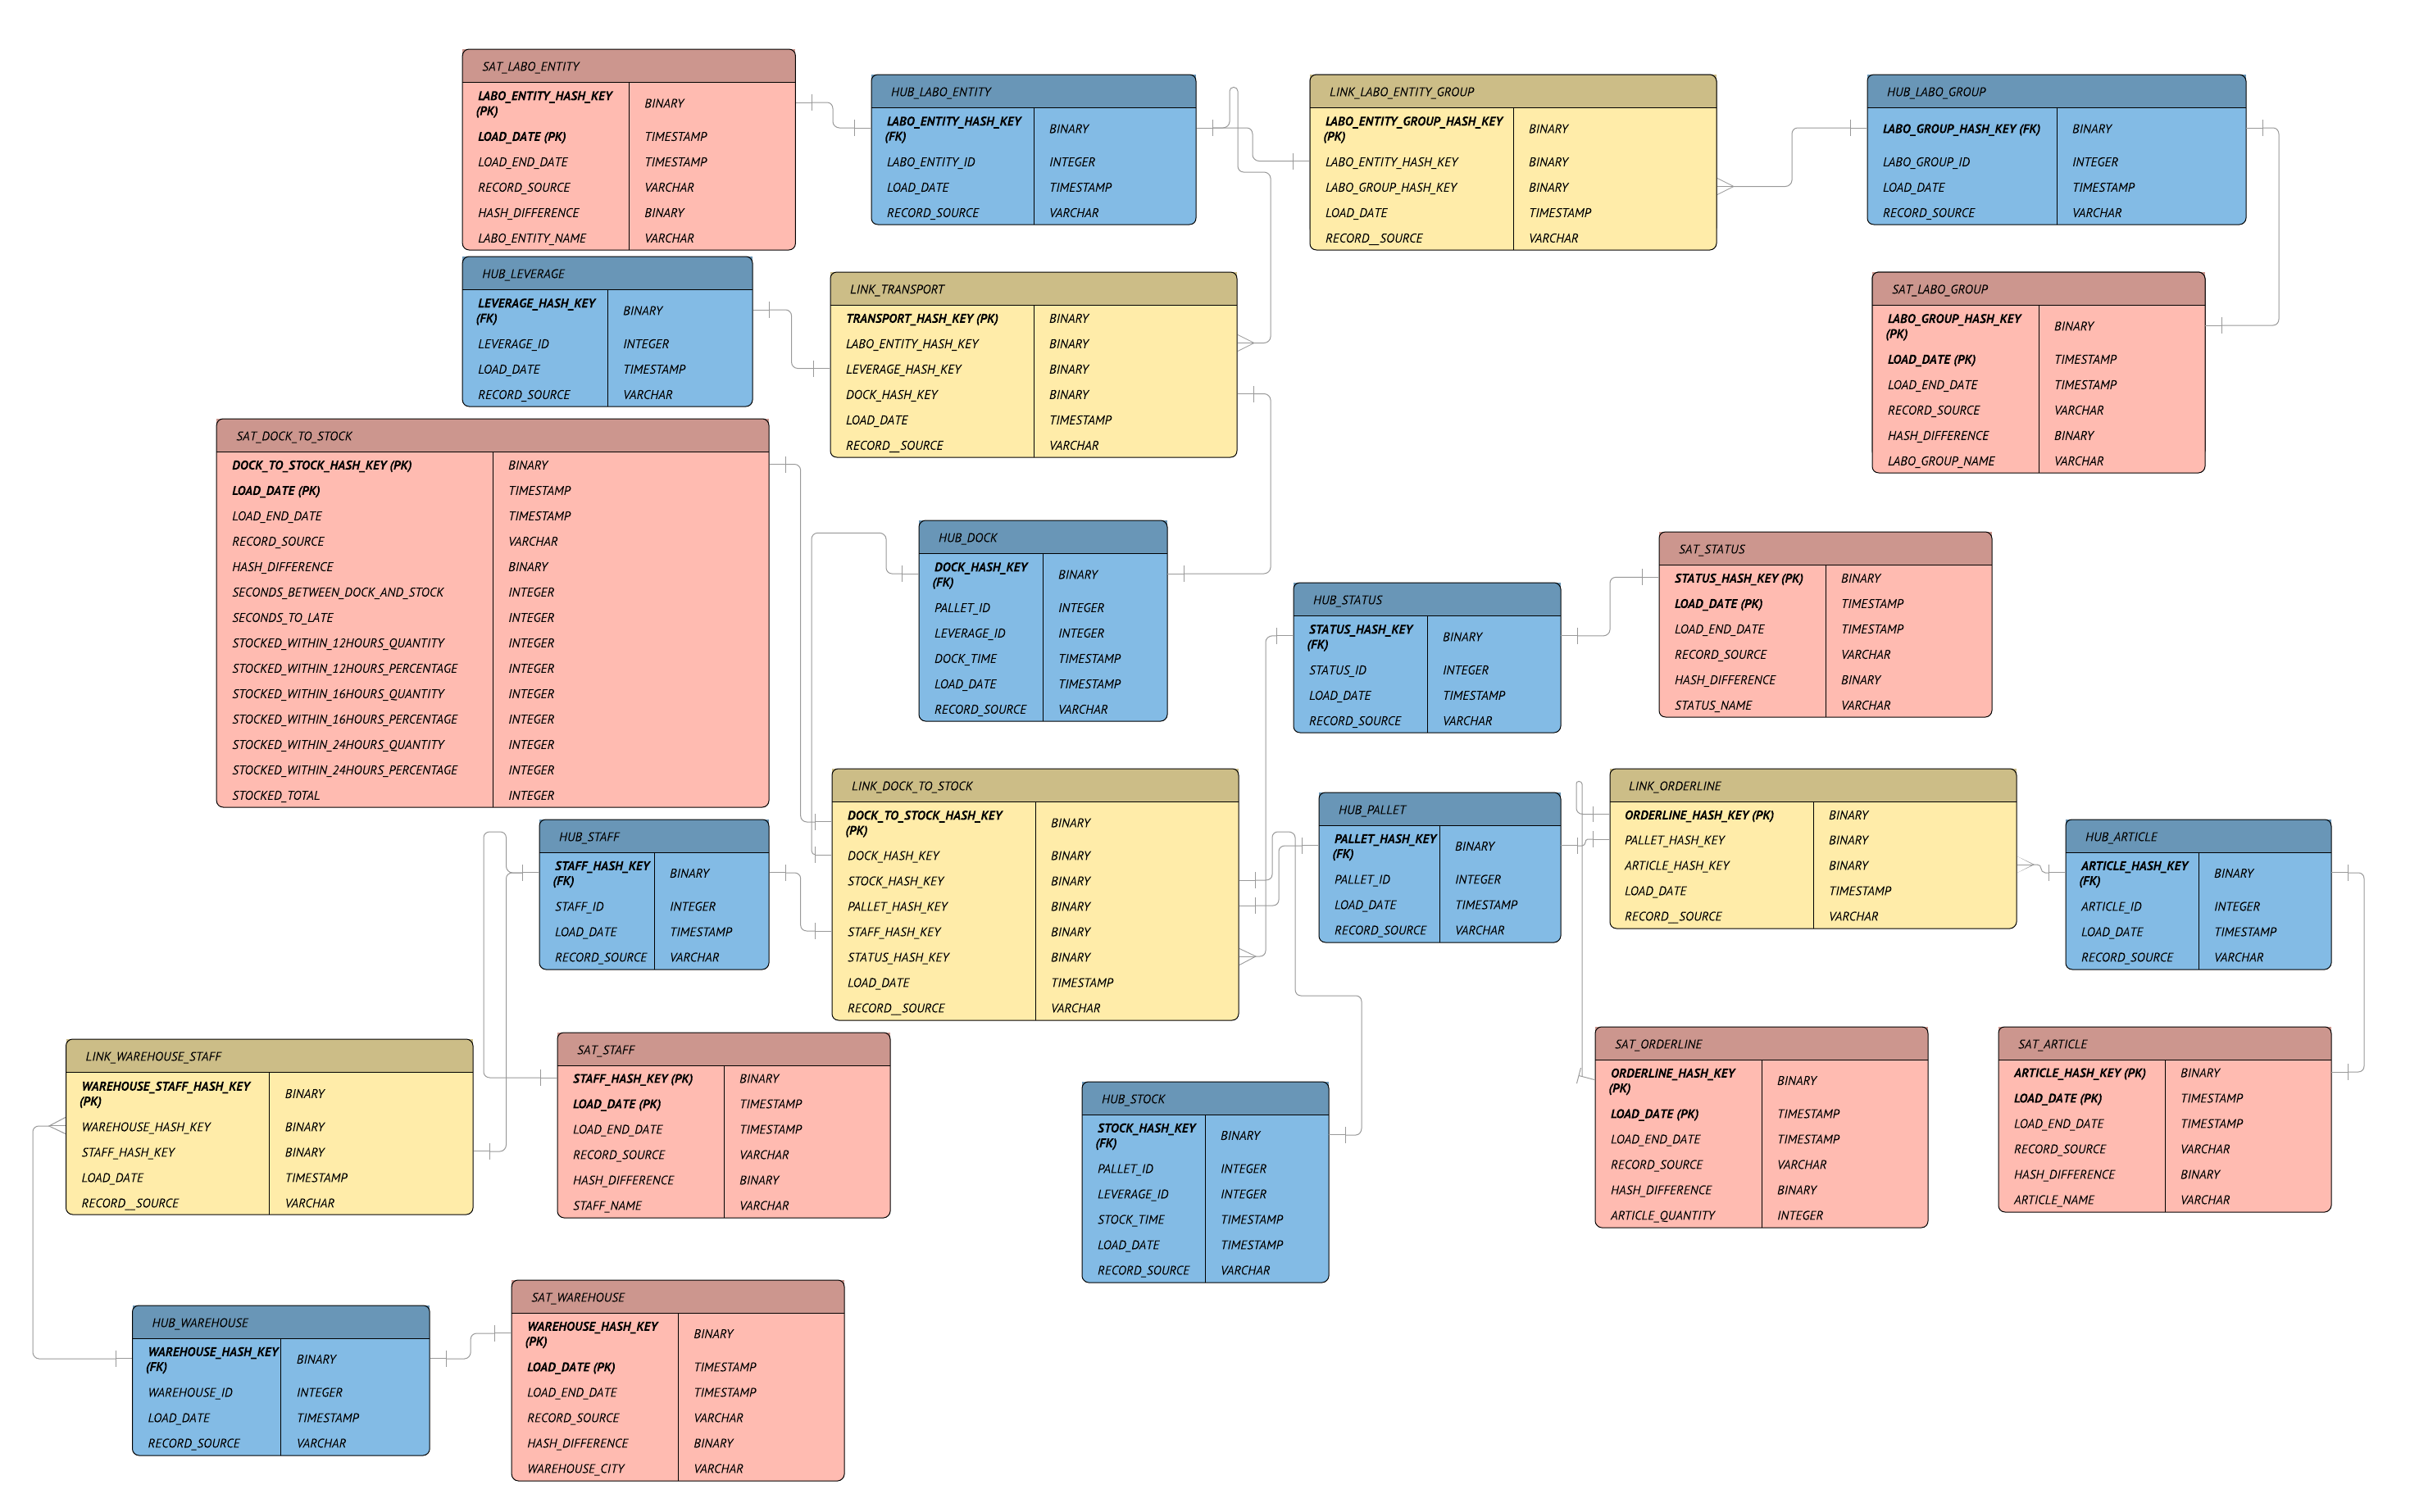
\includegraphics[scale=0.34]{../images/DataVaultModel.png}
	\caption{Voorstelling van het Data Vault model (gemaakt via Lucidchart.com).}
	\label{fig:dvm}
\end{figure}

Het model is opgebouwd uit drie soorten tabellen: de rode entiteiten worden voorgesteld als sattelites, de blauwe entiteiten als hubs en de gele entiteiten vormen de links tussen de verschillende hubs. In de SAT\_DOCK\_TO\_STOCK wordt de berekeningen opgeslagen die nodig zijn voor het berekenen van de KPI. Hash keys worden opgeslagen onder het type ''binary''.

\section{Staging area}
\label{sec:stagareadv}
In de staging area worden alle gegevens in de originele vorm ingeladen. Dit betekent dat hierop nog geen manipulaties mogen gebeuren. In dit onderzoek wordt de data ingeladen via een virtuele tabel, afkomstig van een remote source.

\begin{figure}[h]
	\centering
	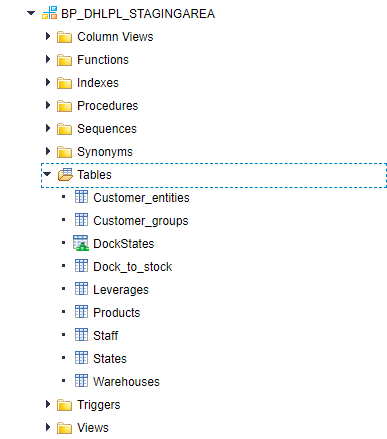
\includegraphics[scale=0.45]{../images/DV_staging.png}
	\caption{Toevoegen van virtuele tabellen aan de staging area.}
	\label{fig:dpa}
\end{figure}

Eens alle virtuele tabellen toegevoegd zijn in de staging area, dan is het modelleren van de eerste laag afgewerkt en kan er overgegaan worden naar het modelleren van de raw data vault.

\section{Opbouw raw data vault}
In de raw data vault wordt de source data omgevormd naar de data vault methodologie. Hierbij wordt nog geen extra business logica en/of berekeningen toegevoegd. Concreet voor dit data model zullen de gegevens getransformeerd worden en doorgeladen worden naar alle tabellen, behalve de tabel SAT\_DOCK\_TO\_STOCK (business logica). De data bij de tabel HUB\_DOCK\_TO\_STOCK kan wel al ingeladen worden, aangezien deze geen business logica bevat (een hub of link bevat nooit business logica).

\subsection{ETL}
In dit deel transformeren we de data naargelang de data vault methodologie en laden we de data in de juiste tabellen. 

\subsubsection{Inladen van data bij een sattelite}
Het inladen \& transformeren van de data bij alle sattelites binnen de raw data vault gebeurt gelijkaardig. In dit voorbeeld wordt het ETL-proces weergegeven van SAT\_ORDERLINE en uitgelegd welke stappen ondernomen moeten worden om de data juist in te laden.
\begin{figure}[h]
	\centering
	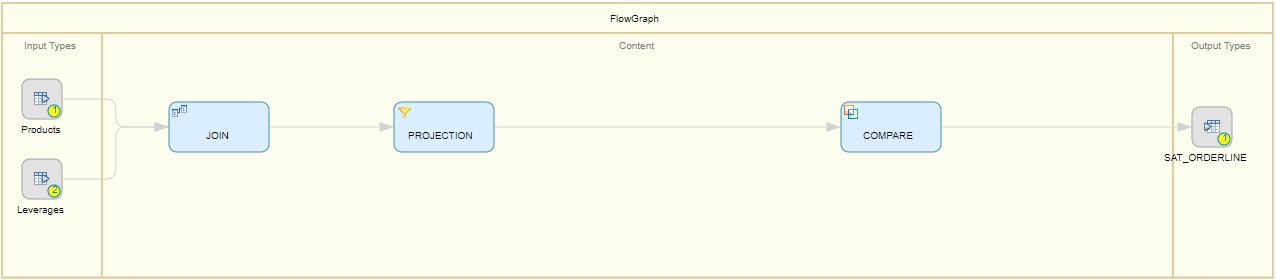
\includegraphics[scale=0.45]{../images/DV_FG_sattelite.png}
	\caption{Een voorbeeld van een ETL proces in SAP HANA bij een sattelite (SAP SDI).}
	\label{fig:etlsat}
\end{figure}
		
In de eerste stap van dit proces worden verschillende bronnen (afkomstig uit de staging area) samengevoegd naar 1 dataset op basis van een gemeenschappelijk attribuut. Alle onnodige data wordt niet meegenomen naar de volgende stap. Deze stap kan ook overgeslagen worden indien de benodigde data afkomstig is uit één bron.

Vervolgens wordt de data getransformeerd naar het juiste formaat (naar het formaat van de destination tabel). Bij de tabel SAT\_ORDERLINE worden volgende manipulaties uitgevoerd:

\begin{itemize}
	\item \textbf{ORDERLINE\_HASH\_KEY (PK):} Een gehashte sleutel van volgende componenten: ''PRODUCT\_ID'' (tabel Products), ''PALLET\_ID'' (tabel Leverages) en de naam van het bronsysteem (in dit geval: ''DATAFILES'').
	\item \textbf{LOAD\_DATE (PK):} Datum/tijdstip wanneer de record geëxtraheerd werd uit de bron.
	\item \textbf{LOAD\_END\_DATE (PK):} Tijdstip tot wanneer de data actueel was, indien deze nog steeds actueel is, krijgt deze de waarde ''9999/12/31 23:59:59'' (belangrijk voor de historiek).
	\item \textbf{RECORD\_SOURCE:} De naam van het bronsysteem waarvan de data afkomstig is (''DATAFILES'' in dit geval).
	\item \textbf{HASH\_DIFFERENCE:} Alle data afkomstig in de entiteit die wordt opgenomen in het data vault model, wordt gehasht naar 1 sleutel. In dit geval wordt enkel ''ARTICLE\_QUANTITY'' versleuteld. 
	\item \textbf{ARTICLE\_QUANTITY:} Het attribuut ''PRODUCT\_QUANTITY'' wordt overgenomen van de brondata.
\end{itemize} 

Nadat de transformaties gebeurd zijn, vergelijken we de nieuwe data met de data die in de destination table zit. Indien de data een nieuwere versies bevat, dan zal deze toegevoegd worden en de ''LOAD\_END\_DATE'' van de oude entiteit gewijzigd worden naar het tijdstip van extractie van de nieuwe entiteit.

\subsubsection{Inladen van data bij een hub}
In elke hub worden de entiteiten bijgehouden die gebruikt zullen worden, en die het meest geschikt zijn voor de rapportering. Deze kunnen ook opgebouwd worden aan de hand van het principe van de "golden record", waarbij de data van verschillende bronnen smaengevoegd worden tot één record, om zo een compleet en correct mogelijke record te verkrijgen. In dit onderzoek is dit niet het geval, aangezien er gewerkt wordt met één bron. 

\begin{figure}[h]
	\centering
	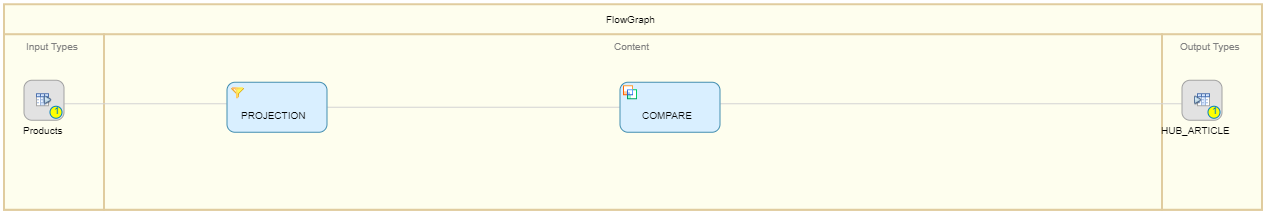
\includegraphics[scale=0.45]{../images/DV_FG_hub.png}
	\caption{Een voorbeeld van een ETL proces in SAP HANA bij een hub (SAP SDI).}
	\label{fig:etlhub}
\end{figure}

Bij de projectie worden volgend transformaties toegepast:

\begin{itemize}
	\item \textbf{ARTICLE\_HASH\_KEY (PK):} Een gehashte sleutel van volgende componenten: ''PRODUCT\_ID'' (tabel Products) en de naam van het bronsysteem (in dit geval: ''DATAFILES'').
	\item \textbf{ARTICLE\_ID:} De business key van de entiteit ''Article'' wordt overgenomen van de brondata.
	\item \textbf{LOAD\_DATE:} Datum/tijdstip wanneer de record geëxtraheerd werd uit de bron.
	\item \textbf{RECORD\_SOURCE:} De naam van het bronsysteem waarvan de data afkomstig is (''DATAFILES'' in dit geval).
\end{itemize}

\subsubsection{Inladen van data bij een link}
Bij het inladen voor de data in de link-entiteiten worden dezelfde stappen doorlopen als bij het inladen van data bij hubs en sattelites. Links stellen de relaties voor tussen de verschillende entiteiten. 

\begin{figure}[h]
	\centering
	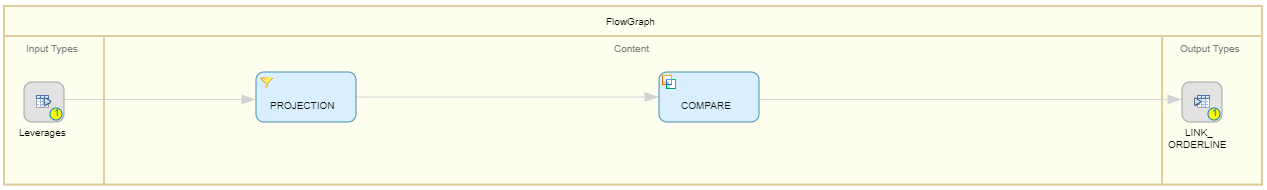
\includegraphics[scale=0.45]{../images/DV_FG_link.png}
	\caption{Een voorbeeld van een ETL proces in SAP HANA bij een link (SAP SDI).}
	\label{fig:etllink}
\end{figure}

\begin{itemize}
	\item \textbf{ORDERLINE\_HASH\_KEY (PK):} Een gehashte sleutel van volgende componenten: ''PRODUCT\_ID'' (tabel Leverages), ''PALLET\_ID'' (tabel Leverages)  en de naam van het bronsysteem (in dit geval: ''DATAFILES'').
	\item \textbf{ARTICLE\_HASH\_KEY:} Een gehashte sleutel van volgende componenten: ''PRODUCT\_ID'' (tabel Leverages).
	\item \textbf{PALLET\_HASH\_KEY:} Een gehashte sleutel van volgende component: ''PALLET\_ID'' (tabel Leverages).
	\item \textbf{ARTICLE\_ID:} De business key van de entiteit ''Article'' wordt overgenomen van de brondata.
	\item \textbf{LOAD\_DATE:} Datum/tijdstip wanneer de record geëxtraheerd werd uit de bron.
	\item \textbf{RECORD\_SOURCE:} De naam van het bronsysteem waarvan de data afkomstig is (''DATAFILES'' in dit geval).
\end{itemize}

\section{Opbouw business vault}
Aangezien de Business vault in dit data schema slechts 1 nieuwe entiteit bevat, verteld de methodologie van data vault dat het niet nodig is om een nieuwe laag hiervoor te ontwerpen. De business vault tabellen mogen dan toegevoegd worden aan de raw data vault indien dit de complexiteit niet aanzienlijk zou verhogen.

Bij het aanmaken van het ETL proces bij een sattelite binnen de Business vault, worden dezelfde stappen overlopen als bij het aanmaken van een sattelite binnen de raw data vault. Bij ''projection'' wordt dan de benodigde business logica en de benodigde berekeningen toegevoegd.

\section{Opbouw data mart}
Wanneer alle data getransformeerd en ingeladen is in de data vault modellen, moeten deze verbonden worden met elkaar en wordt hiervoor een virtuele view aangemaakt waarop verbonden kan worden vanuit een rapporteringsomgeving.

Een best practice die in dit onderzoek werd toegepast was het samenvoegen van alle hubs, links \& sattelites in één dimensie. Zo wordt een beter overzicht behouden van de opgestelde calculation views en wordt de complexiteit verminderd. Deze dimensie werd dan verbonden met een fact table in een sterschema. 

\begin{figure}[h]
	\centering
	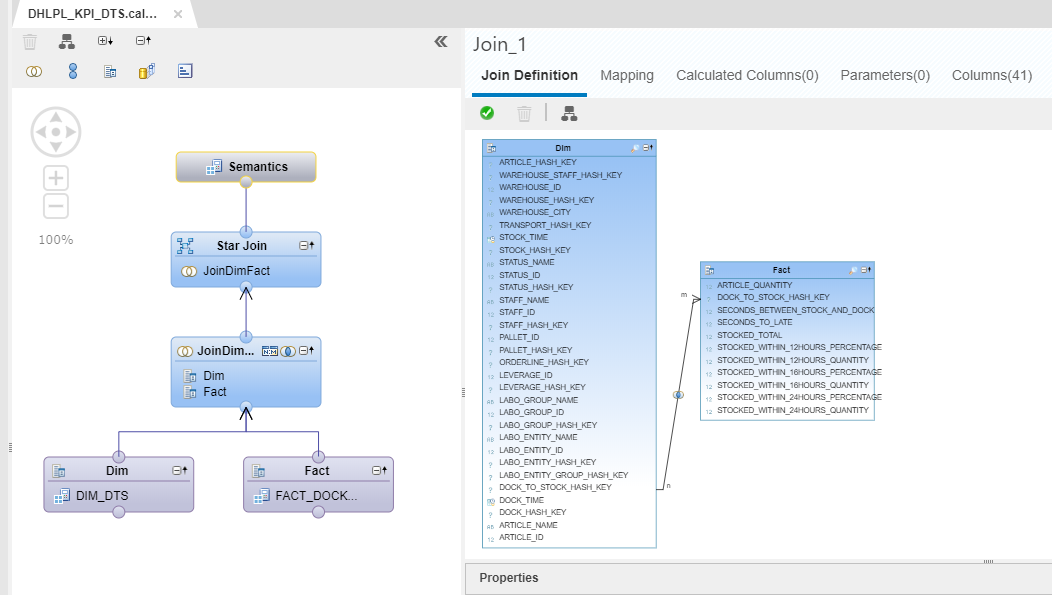
\includegraphics[scale=0.5]{../images/DV_FG_datamart.png}
	\caption{Sterschema opgesteld in SAP voor data vault.}
	\label{fig:dvdm}
\end{figure}
